\chapter{Résultats}
    \section{MemoLanguage}
    \subsection{Recherche}
    \begin{figure}[H]
        \centering
        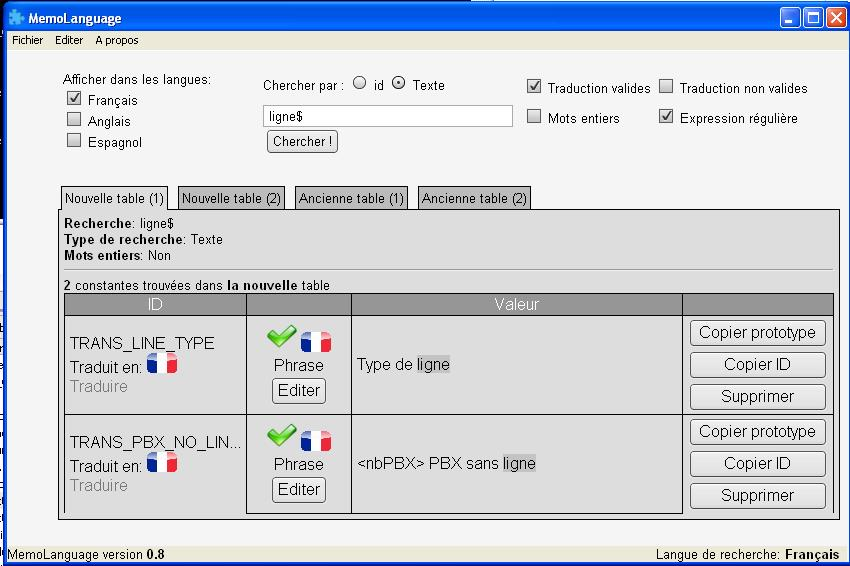
\includegraphics[width=16cm]{images/2-activite/searchRegex.jpg}\label{searchRegex}
        sur cette capture, on peut voir les différentes case à cocher permettant d'affiner la recherche.

            \'Egalement, 4 onglets sont présents, suivant sur l'onglet où on se trouve, cela cherchera dans la nouvelle table ou dans l'ancienne table, comme indiqué par l'onglet.

            La présence de plusieurs onglets, permet de ne pas effacer une recherche qui est intéressante.

        \caption{Recherche avec expression régulière}
    \end{figure}

    \subsection{\'Edition}
        \begin{figure}[H]
            \centering
            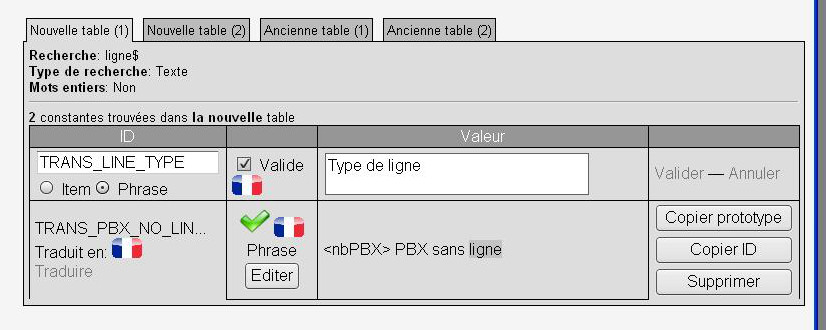
\includegraphics[width=16cm]{images/2-activite/edition.jpg}
            \caption{\'Edition d'une constante}
            \label{edition}
        \end{figure}
    \subsection{Ajout de constante}
    \label{ajoutCst}
        \begin{figure}[H]
            \centering
            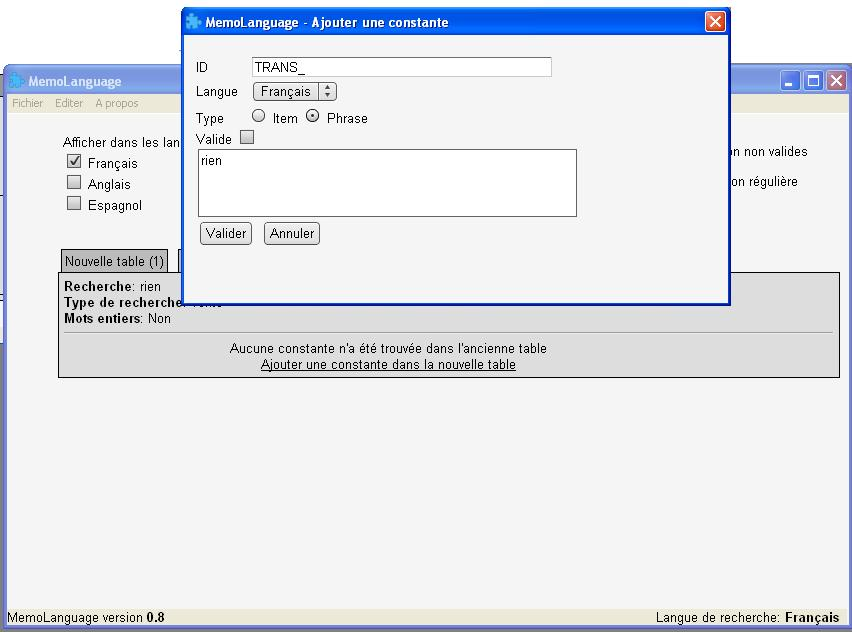
\includegraphics[width=16cm]{images/2-activite/ajoutCst.jpg}

            Sur cette capture d'écran, l'utilisateur à effectuer la recherche ''rien`` et n'a trouvé aucune correspondance, ainsi il a cliquer sur le lient ''Ajouter une constante dans la nouvelle table`` ce qui lui a ouvert la fenêtre avec le champ de valeur pré-remplit avec ''rien``.
            Le nom d'ID est également pré-remplit avec \texttt{TRANS\_} afin d'inciter les développeurs à utiliser ce préfixe.
            \caption{Ajouter d'une constante après une recherche infructueuse}
        \end{figure}
    \subsection{Suppression}
    \label{suppression}
        \begin{figure}[H]
        \centering
        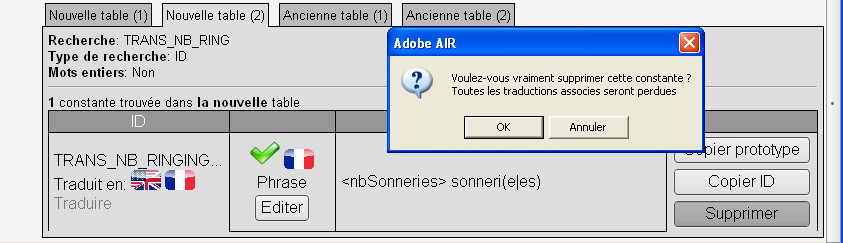
\includegraphics[width=16cm]{images/2-activite/suppression.jpg}
        \caption{Suppression d'une constante}
    \end{figure}
        \subsection{Copier vers nouvelle table}
    \begin{figure}[H]
        \centering
        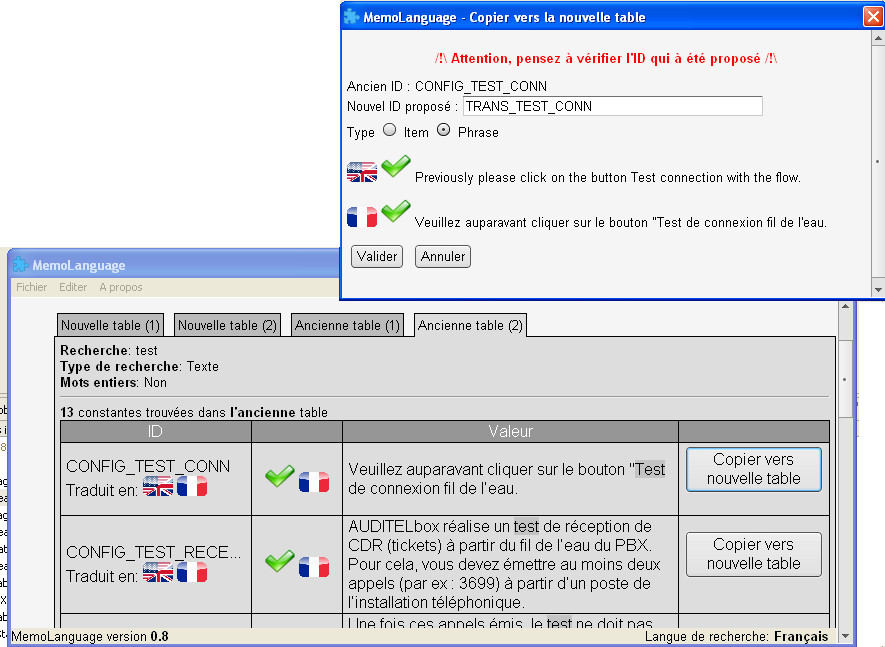
\includegraphics[width=16cm]{images/2-activite/copierVersNouvelleTable.jpg} \caption{Basculer une constante de l'ancienne base vers la nouvelle}
        \label{copierVersNouvelleTable}
        Dans cette capture d'écran, on remarque qu'automatiquement un nouvel ID est proposé afin de garder la cohérence avec les préfixe, cependant une invitation à vérifier et indiquer au développeur.
    \end{figure}

    \subsection{Traduction}
    \label{traduction}
    \begin{figure}[H]
        \centering
        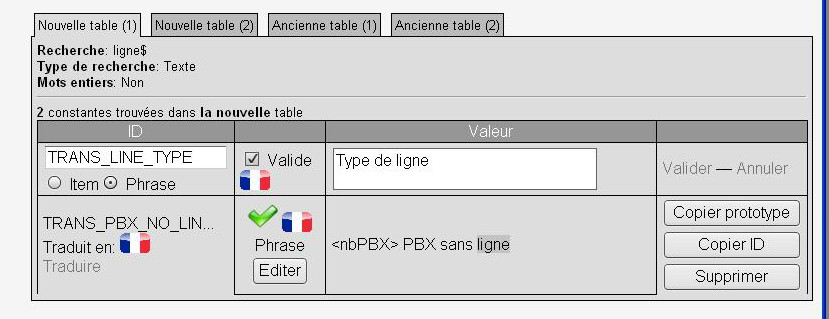
\includegraphics[width=16cm]{images/2-activite/traduction.jpg}
        \caption{Traduction d'une constante}
    \end{figure}

    \subsection{Champs TranslatedText\_short et TranslatedText\_long}
    \label{nouveauxScreens}
        \begin{figure}[H]
        \centering
        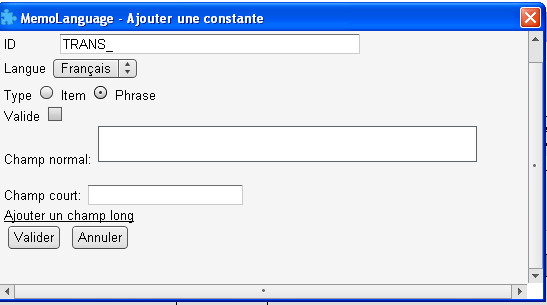
\includegraphics[width=16cm]{images/annexes/resultats/nouvelleInsertion.jpg} 
        \caption{Insertion d'une constante}
        \label{champCourtLong}
    \end{figure}
    \begin{figure}[H]
        \centering
        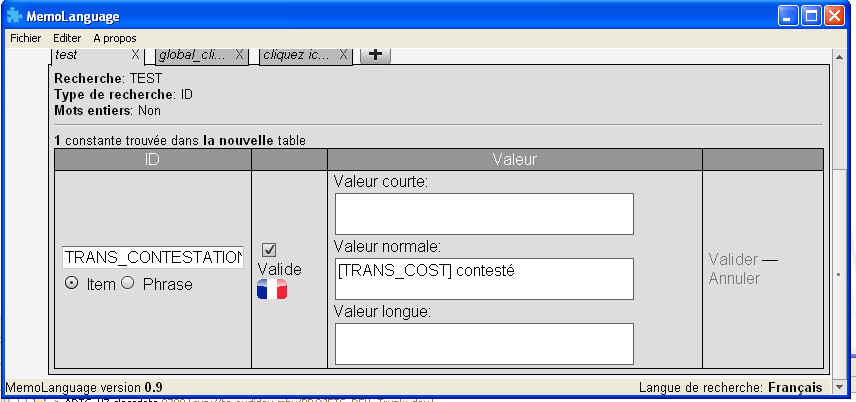
\includegraphics[width=16cm]{images/annexes/resultats/nouvelleEdition.jpg}
        \caption{\'Edition d'une constante}
    \end{figure}
        \section{\adt{} multilingue}
        \begin{figure}[H]
        \centering
        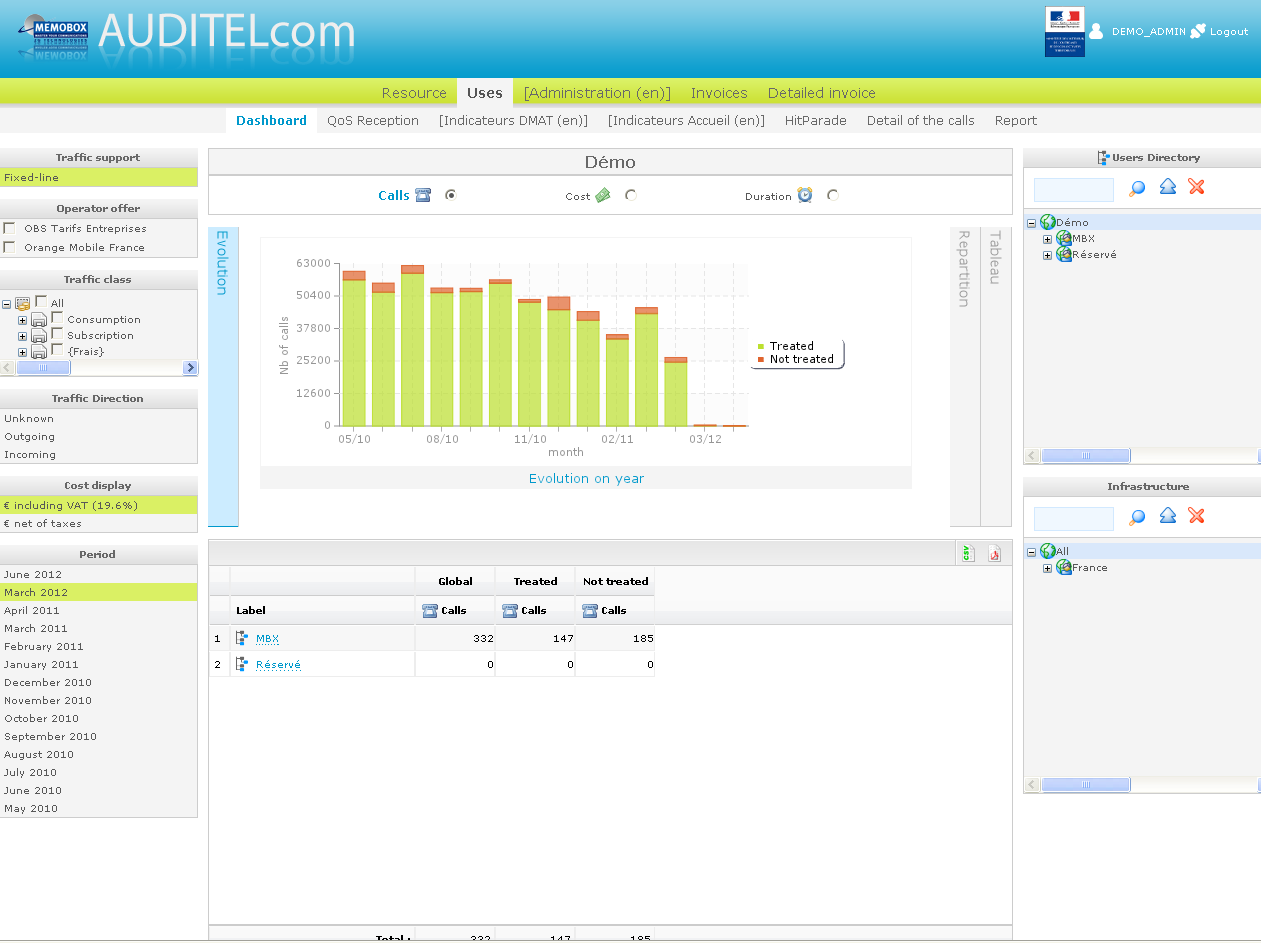
\includegraphics[angle=90,width=16.5cm]{images/annexes/resultats/adtAnglais.png}
        \caption{\adt{} en anglais}
        \label{adtAnglais}
    \end{figure}
            Comme vous pouvez le voir, l'intégration n'est pas finit, certains mots s'affichent en français, cependant une grande partie du travail à été fait.



